\chapter{Design}
This chapter presents the design choices made to address the requirements outlined in \cref{chap:requirements}. The system is composed of several integrated components, as illustrated in \cref{fig:baseArchDiag}, and described in more detail in \cref{fig:fullArchDiag}:
\begin{itemize}
    \item A set of \textit{smart contracts} responsible for all blockchain-related operations, including \acrshort{sw} creation and transaction management (see \cref{sec:smartContractsDesign}).
    \item A \textit{browser extension} that allows students to manage their academic wallets (see \cref{sec:browserExtensionDesign}).
    \item A \textit{\acrfull{sdk}} designed for universities to interact with the \acrshort{ew} system (see \cref{sec:sdkDesign}).
    \item An external \textit{decentralized storage system} used to store and retrieve certification files (see \cref{sec:decStorageDesgn}).
\end{itemize}
\begin{figure}
  \centering
  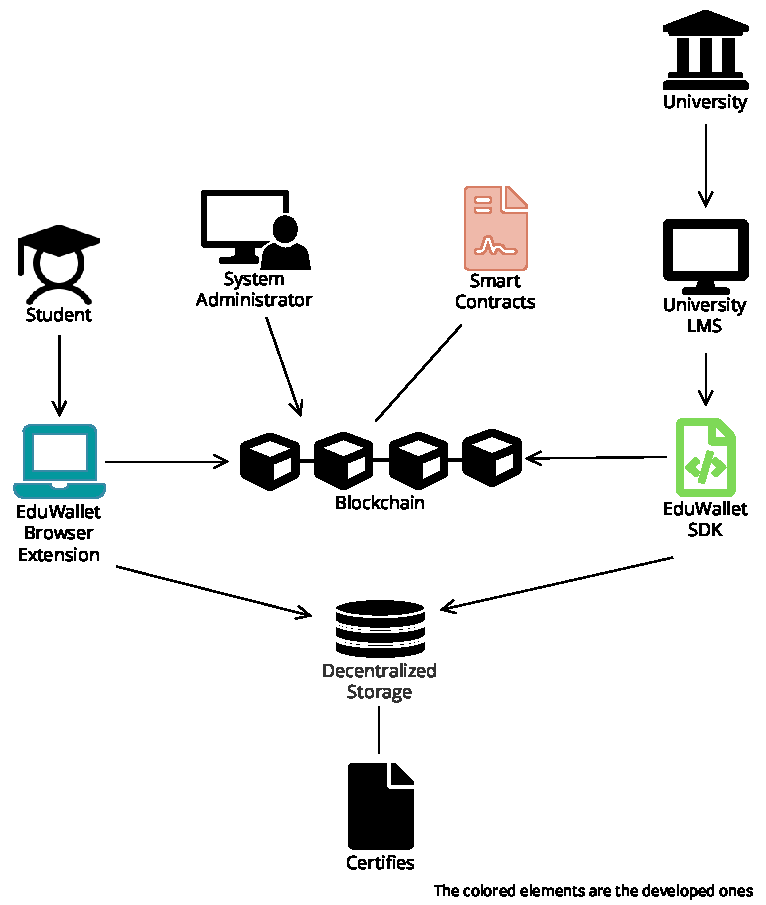
\includegraphics[width=0.6\textwidth]{figures/Architecture diagram basic.pdf}
  \caption[System basic architecture diagram]{Base architecture of the \acrlong{ew} system}
  \label{fig:baseArchDiag}
\end{figure}
In addition to these core components, we developed a simple yet complete \textit{\acrfull{cli}}, which simulates a university's \acrshort{lms} and its interaction with the academic records system. The \acrshort{cli} serves as a testing and demonstration tool and enables users to perform all operations typically available to universities, thereby simplifying the interaction with our \acrshort{sdk}.

Since the focus of our work is on the interaction of universities and students with the academic registry, the system administrator's core functionalities\footnote{The approval and subscription of universities} have been inserted directly in the \acrshort{cli}. This design decision streamlines our use case and reduces unnecessary complexity.

A more detailed analysis of each component is provided in the following sections.

\begin{figure}
  \centering
  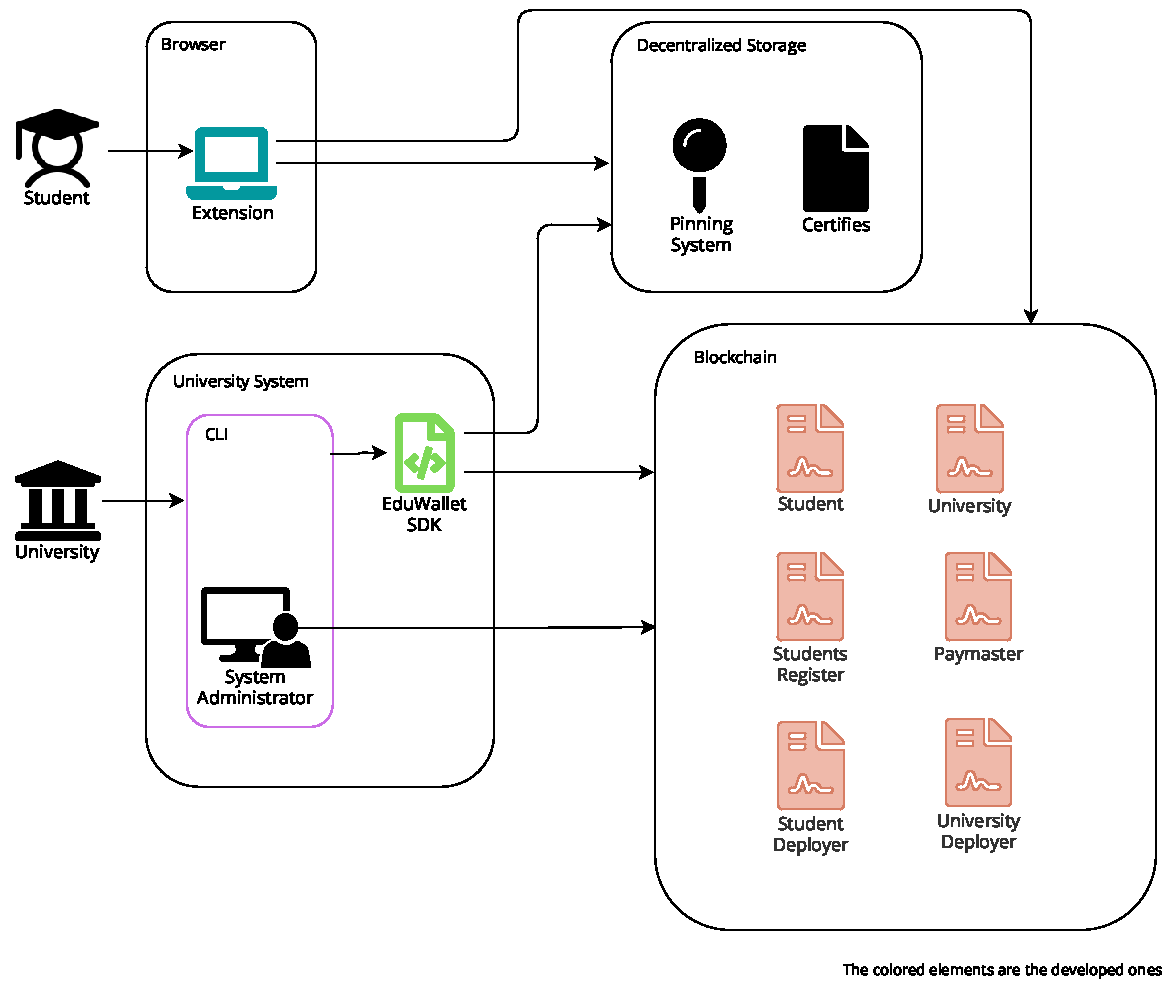
\includegraphics[width=0.8\textwidth]{figures/Architecture diagram complete.pdf}
  \caption[System architecture diagram]{Complete architecture of the \acrlong{ew} system}
  \label{fig:fullArchDiag}
\end{figure}

\section{Smart Contracts}
\label{sec:smartContractsDesign}
In this section we outline the design choices behind the development of the smart contracts. They are the core logic of the \acrshort{ew} system, enabling secure and decentralized management. Leveraging the blockchain principles, such as wallets and transaction, and more sophisticated features, like access control, they manage students and universities account creation and permission, academic records access and management, and data retrieving. The browser extension, as well as the \acrshort{sdk}, interact with them to provide users with the required functionalities, using TypeScript libraries, like \textit{ethers}\footnote{\url{https://docs.ethers.org/v6}}, to easily access them.

\subsection{Blockchain Platform and Technologies}
The blockchain we chose to develop our system is \acrlong{eth}, a public blockchain that can rely on a large community and with different features that works well in an academic record system \cite{mustafa2024publiceduchain}\cite{yassynzhanbolatzhan2021verificationuniversitystudent}. We chose it because allows smart contract development and deployment with different languages. Another important feature of \acrlong{eth} is it is the base for several layer 2 blockchain technologies, which add various functionalities to the mainnet. Some example of layer 2 chain based on \acrlong{eth} are:

\begin{itemize}
    \item Polygon, which offers faster and cheaper transactions compared to the \acrlong{eth} mainnet.
    \item Arbitrum, that enhances scalability while preserving compatibility with Ethereum smart contracts.
    \item ZKsync, a solution that ensures high security and fast finality through the use of validity proofs.
    \item Optimism, that prioritizes simplicity and close integration with the Ethereum ecosystem.
    \item Starknet, which introduces its own high-performance language, Cairo\footnote{\url{https://www.cairo-lang.org/}}, to optimize for zero-knowledge computation.
\end{itemize}
See \cref{chap:layer2links} for the links to all the layer 2 chains.

We was interested in this feature because it allows to develop an \acrlong{eth} mainnet based smart contracts system, which then can be moved to a layer 2 chain to exploit their peculiarities, with not so much effort.

Chosen the chain, we decided to opt for Solidity\footnote{\url{https://soliditylang.org/}} as language to develop our smart contracts. Solidity is an object oriented programming languages, developed to write smart contracts to run on \acrlong{eth} and its \acrshort{evm}, and with some influences from C++, JavaScript and Python\footnote{\url{https://github.com/ethereum/solidity/blob/develop/docs/index.rst}}. It is the most used to write code on the \acrlong{eth} chain, and it can count on a really big community of developer, that helps in finding content on developers forum. We also had a small experience in developing smart contracts in Solidity, therefore, considering also all the reasons presented before, it was the more natural choice.

\subsection{Architecture}
\begin{figure}
  \centering
  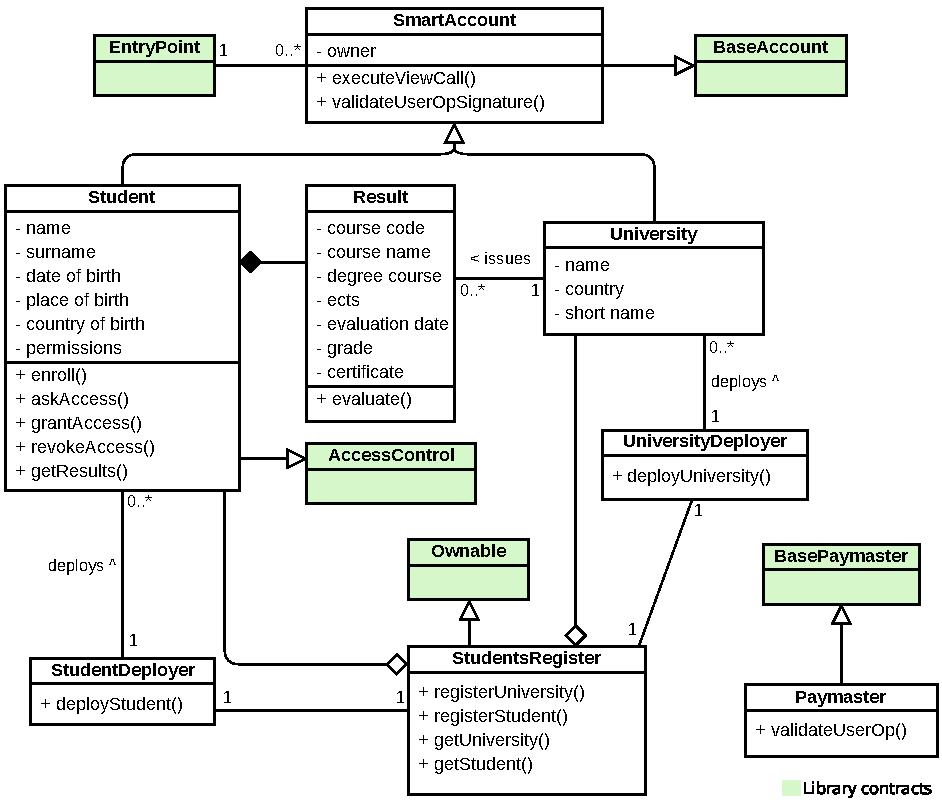
\includegraphics[width=1\textwidth]{figures/Contracts class diagram.pdf}
  \caption[Class diagram showing the smart contracts architecture.]{Smart contracts class diagram}
  \label{fig:contractsClass}
\end{figure}

Leveraging the class diagram shown in \cref{fig:contractsClass}, we are now going to present more in detail the contracts we developed and their functionalities. \acrshort{ew} is composed by seven smart contracts, the white classes in \cref{fig:contractsClass} (\textit{Result} is not a separated smart contract, see \cref{sssec:studentContract} for more details). 

\begin{enumerate}
    \item \textit{SmartAccount}: it defines the structure of a smart account for the account abstraction protocol.
    \item \textit{Student}: smart contract that represents a student.
    \item \textit{University}: used for universities.
    \item \textit{StudentDeployer}: as its name says, it is responsible for the deployment of each \textit{Student} contract.
    \item \textit{UniversityDeployer}: like \textit{StudentDeployer}, it deploys \textit{University} smart contracts.
    \item \textit{StudentsRegister}: it manages and stores the information of students and universities.
    \item \textit{Paymaster}: it funds the transactions of both universities and students.
\end{enumerate}
It exploits also other four contract, the green ones in \cref{fig:contractsClass}, taken from contracts libraries, such as \textit{openzeppelin}:
\begin{enumerate}
    \item \textit{EntryPoint}: singleton contract that receives transactions from smart account, then verifies and executes user operations embedded in them.
    \item \textit{AccessControl}\footnote{\url{https://docs.openzeppelin.com/contracts/5.x/access-control}}: abstract contract that provides a full access control system.
    \item \textit{BaseAccount}: abstract contract that defines the basic behaviour of a smart account in the account abstraction protocol.
    \item \textit{BasePaymaster}: abstract contract that implements the essential structure of a paymaster able to fund users transactions.  
\end{enumerate}


\subsubsection{Student}
\label{sssec:studentContract}

\section{Browser Extension}
\label{sec:browserExtensionDesign}

\section{Software Development Kit}
\label{sec:sdkDesign}

\section{Decentralized Storage System}
\label{sec:decStorageDesgn}
This section presents our solution to one of the most significant challenges in blockchain-based systems: the high cost of on-chain storage. To address this issue, we introduce an off-chain decentralized storage solution in our project. This system is used to store and retrieve certification files, such as language certificates or graduation diplomas, which require significantly more space than plain text\footnote{PDF files typically range from a few kilobytes to several megabytes, whereas plain text data usually occupies only a few bytes.}. Storing such documents directly on-chain would result in substantial gas costs, making the approach impractical. 

\subsection{Why a decentralized storage?}
We chose a decentralized storage system over traditional local or cloud-based solutions to maintain the decentralized nature of our environment and to meet the non-functional requirements outlined in \cref{sec:nonFunctionalRequirements}. Among the various decentralized options available, we selected \acrfull{ipfs} for its ability to provide verifiable and distributed file storage. This choice is motivated by several factors: \acrshort{ipfs} is an open source protocol with a large and active community, strong support, and widespread adoption. It also serves as the foundational layer for many other decentralized platforms, such as Filecoin\footnote{\url{https://filecoin.io}} and Web3.Storage\footnote{\url{https://web3.storage}}, allowing future extensions or upgrades to be implemented with minimal effort \cite{erikflorian2022ipfsandfrineds}. Furthermore, \acrshort{ipfs} ensures immutability of stored files, a critical feature for academic certificates, which must remain unchanged over time.

\subsection{Pinning files}
To fully leverage \acrshort{ipfs}, we integrated Filebase\footnote{\url{https://filebase.com}}, a third-party pinning service. Pinning refers to the act of instructing a node to keep a copy of a file permanently, preventing it from being removed during garbage collection. Without Filebase, we would have needed to run our own local \acrshort{ipfs} node and manage file pinning manually, an approach that introduces instead complexity, higher maintenance costs, and reduced data availability in a testing system like ours. In contrast, Filebase handles node operation and file pinning, offering an accessible solution thorough its AWS S3-compatible \acrshort{api}, which simplifies file uploads to the peer-to-peer network. Notably, Filebase also provides a free tier allowing up to 5 GB of storage, which is sufficient for our needs. This is an advantage over other pinning solutions such as Web3.Storage, which lacks a fully free plan, or Pinata\footnote{\url{https://pinata.cloud}}, which offers more limited options.

\subsection{Integration in the system}
As shown in \cref{fig:fullArchDiag}, both the browser extension and the \acrshort{sdk} interact with the storage system. The browser extension retrieves certificate associated with academic records using the official \acrshort{ipfs} public gateway. It presents students with a direct link to each certificate, composed by the gateway's base \acrshort{url} followed by the file's \acrfull{cid} on the \acrshort{ipfs} network. The \acrshort{cid} of each document is stored on-chain within the student's academic wallet, alongside other record information such as the course name. This enables students to view and download their certificates from a standard web interface.

% TODO: Add photo of the extension where you can see the link of a certification
Similarly, the \acrshort{sdk} uses the same mechanism to retrieve certificates on behalf of universities. When uploading a file, however, the \acrshort{sdk} interacts directly with Filebase to ensure the file is pinned and hosted by an active node. The \acrshort{sdk} receives the document from the university, then uses the AWS S3-compatible \acrshort{api} to upload it. The \acrshort{api} requires the key associated with the pinning account (managed by the \acrshort{ew} system administrator) and the file itself. In return, it provides the \acrshort{cid}, which is then stored in the academic record.
% TODO: Reference implementation section

\subsection{Security and Limitations}
Academic certifies, and official documents more broadly, are legal artifacts that must always be secure and verifiable. \acrshort{ipfs} inherently supports these properties through its use of content-based addressing. In this model, each file is identified by a \acrshort{cid}, which is derived from the cryptographic hash of the file's content. Any alteration to the file results in a completely different \acrshort{cid}, ensuring that tampering is immediately detectable \cite{benet2014ipfscontentaddressed}. Since the the \acrshort{cid} is stored on the blockchain at the time the certificate is issued by the university, the document's authenticity and integrity are guaranteed.

While \acrshort{ipfs} offers strong immutability and verifiability, it lacks built-in access control. In the context of our system, we assume that certificates are publicly accessible documents. Consequently, any part in possession of a file's \acrshort{cid} can retrieve it via the public gateway. However, if access control becomes a requirement, there are several strategies to address this limitation \cite{barbaraanrealaura2021datapersistence}. One option is to encrypt files before uploading them to \acrshort{ipfs}, such that only authorized components within our system can decrypt them. Another approach is to use a private \acrshort{ipfs} network, where access can be restricted to approved entities. The trade-offs and potential implications of such private deployment will be discussed in the FUTURE WORK CHAPTER.

\section{CLI}
\label{sec:cliDesign}
\begin{figure}
  \centering
  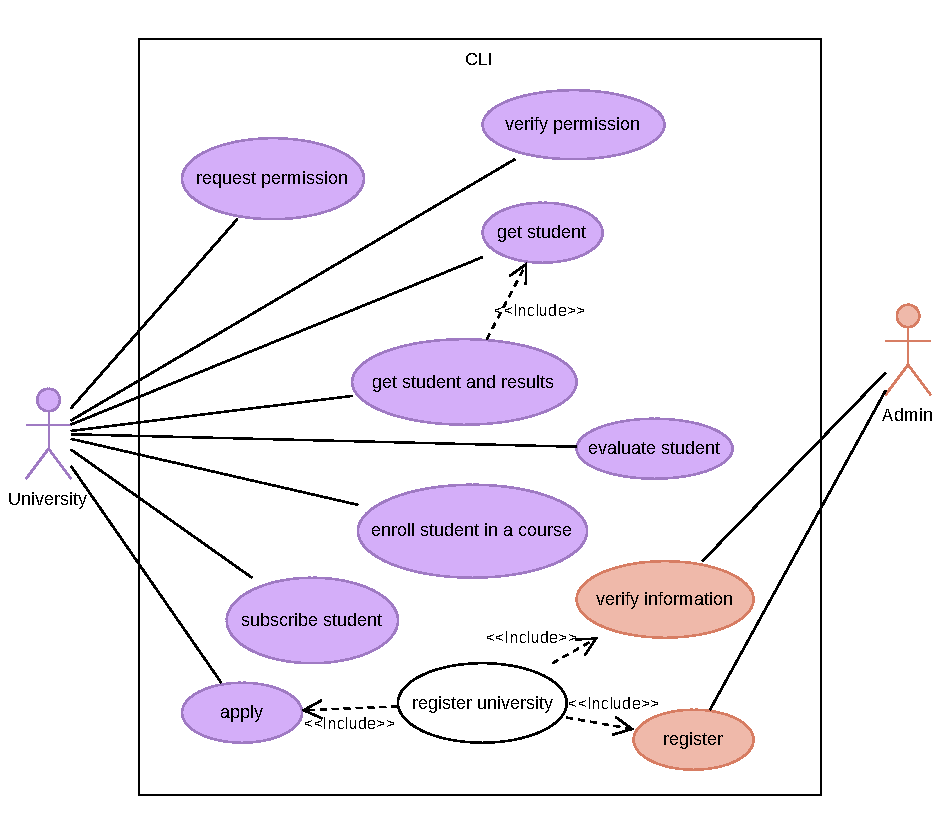
\includegraphics[width=0.8\textwidth]{figures/CLI use case diagram.pdf}
  \caption[Use case diagram representing the functionalities provided by the \acrshort{cli}.]{\acrshort{cli} functionalities}
  \label{fig:useCaseCli}
\end{figure}
This section describes the testing tool developed to evaluate the use of the \acrshort{sdk}. In a real-world deployment, universities are expected to integrate the \acrshort{sdk} into their existing \acrshort{lms} to interact with \acrlong{ew}. However, given that this is a testing environment, smaller and simpler than a real-world deployment, we developed a minimal \acrlong{cli} to simulate the interaction between a university's system and our academic register. We opted to implement a CLI rather than a web application or desktop GUI and this decision allowed for faster development, enabling us to focus on the core functionalities of the \acrshort{sdk}, the blockchain logic, and the browser extension, without introducing additional complexity related to graphical or \acrfull{ux} design.

\cref{fig:clifigs} illustrates the visual aspects of the \acrshort{cli}. In \cref{sfig:cliDesign1}, users can navigate through a sliding menu offering various options. When input is required, the interface prompts the user for the necessary information and provides visual feedback upon completion of the operation (\cref{sfig:cliDesign2}).The \acrshort{cli} leverages the \textit{inquirer}\footnote{\url{https://www.npmjs.com/package/inquirer}} TypeScript library to manage user interactions and uses \textit{ora}\footnote{\url{https://www.npmjs.com/package/ora}} to display feedback. Specifically, \textit{ora} is responsible for showing success and error messages, as well as animated text with spinners to indicate ongoing operations.

\begin{figure}
    \centering
    \begin{subfigure}{.5\textwidth}
        \centering
        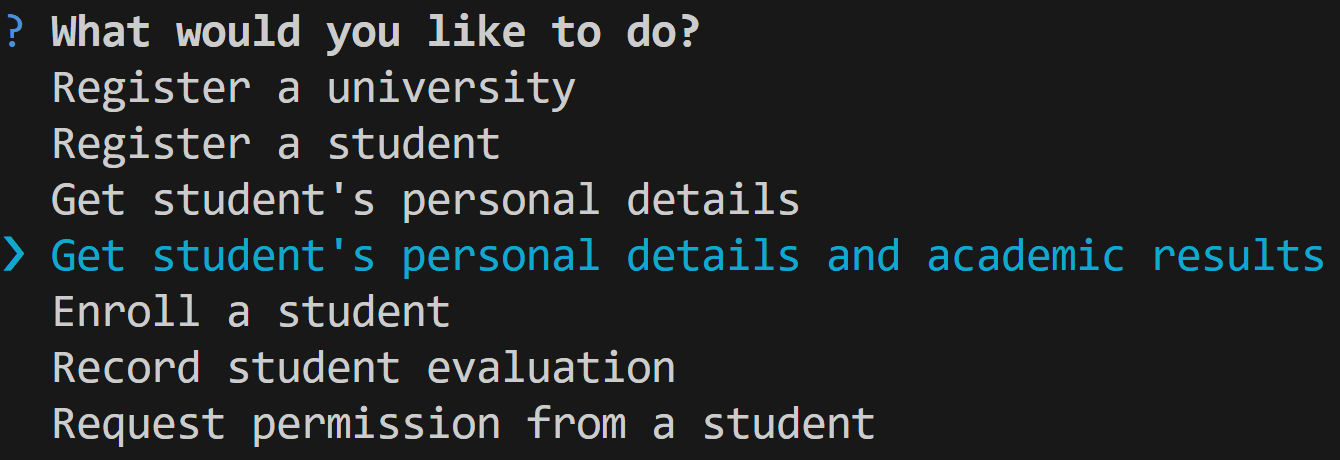
\includegraphics[width=\textwidth]{figures/CLI screen 1.png}
        \caption{Sliding menu}
        \label{sfig:cliDesign1}
    \end{subfigure}
    \hfill
    \begin{subfigure}{.60\textwidth}
        \centering
        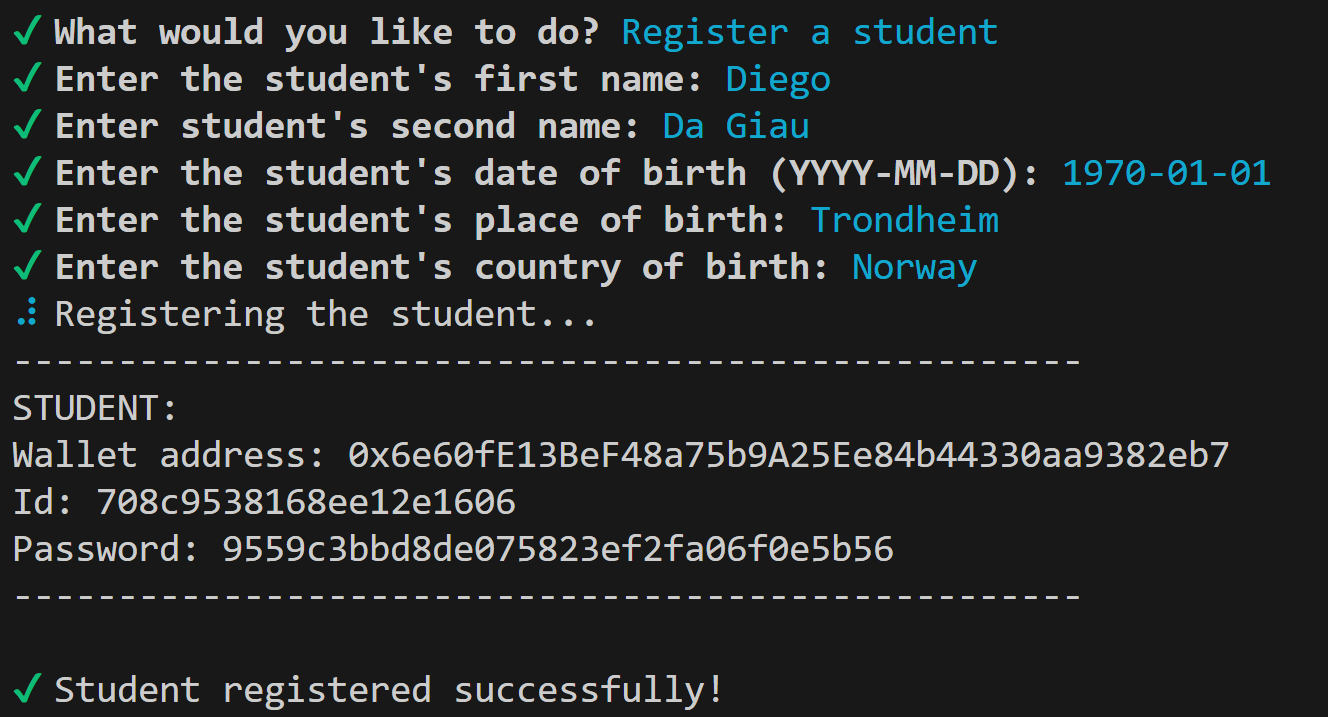
\includegraphics[width=\textwidth]{figures/CLI screen 2.png}
        \caption{User input and visual feedbacks}
        \label{sfig:cliDesign2}
    \end{subfigure}
    \caption[Group of images showing different aspects of the \acrshort{cli} interface.]{Different aspects of the \acrshort{cli} interface}
    \label{fig:clifigs}
\end{figure}

\subsection{Functionalities}
The \acrshort{cli} exposes all the functionalities outlined in \cref{fig:useCaseCli}. Users can:
\begin{itemize}
    \item Submit a request to register a university in the \acrshort{ew} system.
    \item Register a new student.
    \item Retrieve a student’s personal details.
    \item Retrieve a student’s details and academic results.
    \item Enrol a student in a new course.
    \item Evaluate a student.
    \item Request permissions from a student.
    \item Verify existing permissions.
\end{itemize}
Additionally, the \acrshort{cli} provides options to change the current university and exit the program.

\subsubsection{Testing environment initialization}
Before performing any operation, the \acrshort{cli} must initialize a local blockchain test network by deploying the following smart contracts:
\begin{itemize}
    \item \textit{EntryPoint}
    \item \textit{StudentDeployer}
    \item \textit{UniversityDeployer}
    \item \textit{Paymaster}
    \item \textit{StudentsRegister}
\end{itemize}
The \textit{Paymaster} contract then must also be funded to sponsor transactions on behalf of users.

In public testnets or in production networks, this step would be unnecessary, as the contracts would already be deployed. Their addresses would be hardcoded in the \acrshort{cli}, \acrshort{sdk} and browser extension.

\subsubsection{University registration}
\label{sssec:applyEw}
To apply to the \acrshort{ew} system, a university must provide its name, country, and short name. Upon completion, it receives the private key of the wallet that owns its smart account. This key is used by the \acrshort{cli} to generate the university's \acrlong{eth} wallet, which is then stored as the current active university. In a real \acrshort{lms}, the private key must be securely stored and used to initialize the wallet and use the \acrshort{sdk}. 

To interact with the \textit{EntryPoint}  contract in the local testnet, the \acrshort{cli} also funds the university's \acrshort{eth} wallet. In public or production networks, this is not necessary, as the bundler pays the transaction fees and is reimbursed by the \textit{Paymaster}.

\subsubsection{Register a new student}
To register a student, the  university provides their name, surname, date of birth, place of birth and country of birth. The \acrshort{cli} then calls the \acrshort{sdk} to create the student's academic wallet and credentials, which are returned to the university (\cref{sfig:cliDesign2}). The academic wallet address uniquely identifies the student and must be stored by the university, as it is required for all future interactions. 

As discussed in the CONTRACT SECTION, universities are responsible for registering students to decentralize the validation process. Since universities already verify student applications, they can provide verified data to the system, avoiding centralization and overloading the system administrator.

The \acrshort{cli} also funds the student's \acrlong{eth} wallet  for local testing. The wallet address is obtained from the login credentials, as done in the browser extension (see BROWSER EXTENSION SECTION).

\subsubsection{Student Information Retrieval}
To retrieve a student's personal information or full academic record, university must provide the student's academic wallet address. The \acrshort{cli} then returns the requested data.

\subsubsection{Enrol and evaluate}
To enrol or evaluate a student, the university must provide the academic wallet address and course code. Enrolment also requires the course name, number of \acrshort{ects} and degree course name (e.g., \textit{Master's in Computer Engineering}, or \textit{Bachelor's in Biology}). Evaluation requires the evaluation date and, optionally, the path to a certificate file. Since the \acrshort{sdk} allows enrolment in or evaluation of multiple courses at once, the \acrshort{cli} also supports submitting multiple records in a single command.     

\subsubsection{Permissions: Request and Verification}
To access or modify student's academic records, the university must request permission. The \acrshort{cli} requires the student's wallet address and the type of permission (read or write). As in most systems, write permission implies read access.
The \acrshort{cli} also includes an option to verify whether the university currently has read or write permission for a specific student.

\subsubsection{Changing University and Exiting the \acrshort{cli}}
These functionalities are unique to the \acrshort{cli} and are included for convenience. To change the active university, the user provides the private key of another registered university. To exit the \acrshort{cli}, the user selects the corresponding menu option.

\subsubsection{Administrator Functionalities}
The \acrshort{cli} also includes admin functionalities, to facilitate system testing. Specifically, the administrator can:
\begin{itemize}
    \item Review the information submitted in university registration request.
    \item Approve and register universities in the system.
\end{itemize}
These functionalities are embedded within the university registration option. A university is automatically registered when its information is provided by the user during the registration process.

\subsection{Data validation}
All user input is validated using regular expressions and formatting rules. For instance, wallet addresses and private keys are validated based on length and structure\footnote{Private keys must start with \textit{0x} and be followed by 64 hexadecimal characters; addresses by 42.}. Strings are validated to fall within predefined length limits. Dates must follow the \textit{YYYY-MM-DD} format to avoid ambiguity and must be after January 1, 1970, as they are stored as Unix timestamps (unsigned integers). \acrshort{ects} values are checked to ensure they are valid integers or floating-point numbers within acceptable limits. Since the smart contracts store \acrshort{ects} as integers scaled by 100 (to avoid the issue of Solidity with floating point numbers), the \acrshort{cli} ensures the values will not cause overflow during storage.